\chapter{Desenvolvimento}\label{sec:desenvolvimento}

Esta seção tem como objetivo apresentar o processo de desenvolvimento da proposta atual, fundamentado nas etapas previamente descritas na seção de metodologia. Serão discutidos também os desafios encontrados durante o processo e possíveis ajustes na direção do projeto à medida que obstáculos emergem.

O processo de desenvolvimento da proposta inicia com a etapa de Mapeamento, na qual serão definidos os requisitos, formuladas as perguntas de pesquisa, realizado o mapeamento sistemático da literatura e estabelecidos os requisitos não funcionais para acessibilidade.

Em seguida, na etapa de Modelagem, serão construídos o Diagrama de Sequência, o Diagrama de Componentes, o Modelo Lógico de Dados e o Diagrama de Classes. Esses diagramas e modelos servirão como alicerce para a próxima fase.

Na fase do Projeto, será projetada a arquitetura de integração com o Flutter e selecionados os frameworks, bibliotecas e linguagens que serão usados no desenvolvimento da ferramenta.

Com a conclusão da etapa de Projeto, o processo de Desenvolvimento será iniciado, onde serão aplicados Padrões de Projeto e Expressões regulares, além de preparar a ferramenta para publicação.

Após a conclusão do desenvolvimento, a etapa de Testes será iniciada. Nela, será adotado o TDD, serão realizados Testes de Unidade e de Integração, bem como Testes dos Requisitos não funcionais de Acessibilidade.

Finalmente, na etapa de Validação, será realizada uma pesquisa com desenvolvedores e pessoas com deficiência, aplicado o SUS e executada uma prova de conceito. Essa etapa final permitirá avaliar a eficácia da ferramenta desenvolvida e identificar áreas de melhoria potencial. Cada uma dessas etapas será discutida em detalhes nas seções subsequentes deste capítulo.

\section{Mapeamento Inicial}

O processo inicial de mapeamento é fundamental para a abordagem de identificação dos Requisitos Funcionais (RF), Requisitos Não Funcionais (RNF) e Regras de Negócio (RN).

Os Requisitos Funcionais (RF) são destinados a descrever as funcionalidades que o sistema deve incorporar para atender às necessidades do usuário final. Estes requisitos são essencialmente as ações que o sistema deve ser capaz de realizar, como por exemplo, processar entradas de dados, realizar operações e fornecer saídas de informações.

Por outro lado, os Requisitos Não Funcionais (RNF) definem o conjunto de critérios que orientam o modo como o sistema operará, como as restrições e propriedades desejáveis do sistema que não estão diretamente relacionadas com o comportamento específico dele. Eles estabelecem um escopo com características particulares que o sistema a ser desenvolvido deverá seguir, tais como padrões de projeto, usabilidade, segurança, desempenho, entre outros. Em outras palavras, os RNF são os atributos de qualidade do sistema que determinam como os requisitos funcionais devem ser implementados.

As Regras de Negócio (RN), por sua vez, são diretrizes que definem ou restringem algum aspecto do negócio. Elas descrevem os detalhes das funcionalidades que o sistema deve possuir, para que estas possam ser implementadas de forma a não causar prejuízos a outras funcionalidades. Elas fornecem uma compreensão clara de como o sistema deve se comportar em determinadas circunstâncias e auxiliam na garantia de que o sistema esteja alinhado com as metas e estratégias do negócio.

Em suma, a identificação e compreensão desses três elementos - RF, RNF e RN - são cruciais para o sucesso do desenvolvimento do sistema, garantindo que ele seja construído de acordo com as necessidades do negócio e dos usuários, além de cumprir com os critérios de qualidade estabelecidos.

\subsection{Requisitos Funcionais}\label{sec:requisitos-funcionais}

Os Requisitos Funcionais (RF) identificados para o sistema proposto são:

\newcounter{rf} 
\renewcommand{\therf}{RF\arabic{rf}}

\begin{table}[!htbp]
	\centering
	\renewcommand{\arraystretch}{1.1}
	\caption{Requisitos Funcionais do TCC}
	\label{tab:tabela-requisitos-funcionais}
	\begin{tabular}{ L{2cm}  L{12cm} }
		\hline
		Requisito & Descrição \\
		\hline
		\refstepcounter{rf}\therf\label{req:visualizar-inconsistencia}	& O sistema deve permitir a visualização de inconsistências no código \\
    \refstepcounter{rf}\therf\label{req:marcar-inconsistencia}	& O sistema deve realizar marcações no código baseado na especificação definida \\
    \refstepcounter{rf}\therf\label{req:sugerir-remover-inconsistencia}	& O sistema deve sugerir remover trechos de código baseado na especificação definida \\
    \refstepcounter{rf}\therf\label{req:sugerir-correcao-automatica} & O sistema deve sugerir correções automáticas baseado na especificação definida \\
    \refstepcounter{rf}\therf\label{req:consultar-requisitos} & O sistema deve permitir o usuário consultar todos os requisitos não funcionais de acessibilidade \\
    \refstepcounter{rf}\therf\label{req:desabilitar-requisitos} & O sistema deve permitir o usuário desabilitar requisitos não funcionais de acessibilidade \\
    \refstepcounter{rf}\therf\label{req:linha-comando} & O sistema deve permitir a utilização em ambientes de integração contínua \\
		\hline
	\end{tabular}
	\vspace{2mm}
	\fonte{\me{2023}}
\end{table}

Dos requisitos funcionais da tabela \ref{tab:tabela-requisitos-funcionais}, destaca-se a necessidade de analisar código escrito na linguagem Dart, isso depende de uma ferramenta capaz de processar e interpretar o código fonte da aplicação desenvolvida com Flutter. A equipe do Dart provê uma API para análise estática de código, que será utilizada através do plugin \href{https://pub.dev/packages/analyzer}{analyzer}. Ele já provê uma interface para acessar a árvore sintática abstrata do código fonte, que será utilizada para identificar e marcar as inconsistências no código.

\subsection{Requisitos Não Funcionais}\label{sec:requisitos-nao-funcionais}

Os Requisitos Não Funcionais (RNF) identificados para o sistema proposto são:

\newcounter{rnf}
\renewcommand{\thernf}{RNF\arabic{rnf}}

\begin{table}[!htbp]
	\centering
	\renewcommand{\arraystretch}{1.1}
	\caption{Requisitos Não Funcionais do TCC}
	\label{tab:tabela-requisitos-nao-funcionais}
	\begin{tabular}{ L{2cm}  L{12cm} }
		\hline
		Requisito & Descrição \\
		\hline
		\refstepcounter{rnf}\thernf\label{rnf:utiliza-dart}	& O sistema deve ser escrito utilizando a linguagem Dart \\
		\refstepcounter{rnf}\thernf\label{rnf:pub-dev}	& O sistema deve ser publicado no repositório \href{https:\\pub.dev}{pub.dev} \\
		\refstepcounter{rnf}\thernf\label{rnf:melhores-praticas}	& O sistema deve seguir as melhores práticas para pacotes publicados no repositório \href{https:\\pub.dev}{pub.dev} \\
    \refstepcounter{rnf}\thernf\label{rnf:licenca-aberta}	& O sistema deve possuir licença aberta para permitir alterações e melhorias \\
    \refstepcounter{rnf}\thernf\label{rnf:documentacao}	& O sistema deve possuir documentação para auxiliar na criação de novas regras de negócio de usabilidade \\
		\hline
	\end{tabular}
	\vspace{2mm}
	\fonte{\me{2024}}
\end{table}

Dos requisitos funcionais descritos na tabela \ref{tab:tabela-requisitos-nao-funcionais}, destaca-se a necessidade de seguir as melhores práticas para pacotes publicados no repositório \href{https:\\pub.dev}{pub.dev}. Isso é importante para garantir que o sistema seja facilmente acessível e utilizável por outros desenvolvedores, além de manter a qualidade e a segurança do código fonte. A equipe do Dart provê um guia de boas práticas para publicação de pacotes no repositório \href{https:\\pub.dev}{pub.dev}, que será seguido para garantir a qualidade e a segurança do sistema. Ele também é uma das formas que o repositório classifica plugins auxiliando na escolha dos usuários.

\subsection{Regras de Negócio}\label{sec:regras-negocio}

As Regras de Negócio (RN) identificadas para o sistema proposto são:

\newcounter{rn} 
\renewcommand{\thern}{RN\arabic{rn}}

\begin{table}[!htbp]
	\centering
	\renewcommand{\arraystretch}{1.1}
	\caption{Regras de negócio do TCC}
	\label{tab:tabela-regras-de-negocio}
	\begin{tabular}{ L{2cm}  L{12cm} }
		\hline
		Regra de Negócio & Descrição \\
		\hline
		\refstepcounter{rn}\thern	& As regras de acessibilidade devem ser separadas por pastas para organização clara e simplificada \\
    \refstepcounter{rn}\thern	& Cada regra de acessibilidade deve possuir testes automatizados para validar seu funcionamento \\
    \refstepcounter{rn}\thern	& Cada regra de acessibilidade deve possuir uma descrição clara e objetiva para facilitar a compreensão do desenvolvedor \\
    \refstepcounter{rn}\thern	& Cada regra de acessibilidade deve possuir uma sugestão de correção \\
    \refstepcounter{rn}\thern	& Cada regra de acessibilidade deve possuir uma marcação no código para indicar a inconsistência \\
    \refstepcounter{rn}\thern & As marcações devem ser na cor Laranja, uma vez que a cor vermelha é utilizada para erros de compilação \\
		\hline
	\end{tabular}
	\vspace{2mm}
	\fonte{\me{2024}}
\end{table}

Além das regras de negócio listadas na tabela \ref{tab:tabela-regras-de-negocio}, destaca-se a necessidade de separar as regras de acessibilidade por pastas para organização clara e simplificada. A ideia inicial era utilizar um Mapeamento Sistemático da Literatura para identificar as regras de acessibilidade mais utilizadas e criar um conjunto de regras de acessibilidade padrão. Porém, conforme será descrito nos próximos capítulos, não foi possível levantar um conjunto de regras de acessibilidade padrão, então optou-se por criar um conjunto de regras de acessibilidade baseado nas recomendações de ambas as plataformas.

\section{Modelagem}

Com os requisitos identificados, a próxima etapa é a Modelagem, onde serão construídos os diagramas e modelos que servirão como base para o desenvolvimento do sistema.

\subsection{Diagrama de Sequência}

Diagramas de sequência são diagramas de interação que mostram como grupos de objetos colaboram em algum comportamento ao longo do tempo. Eles são usados para capturar o comportamento de um único caso de uso, ou seja, um cenário específico de interação entre objetos.

O diagrama de sequência da figura \ref{fig:diagrama-sequencia-plugin} a seguir ilustra a interação básica do desenvolvedor com o plugin:

\begin{figure}[!ht]
	\centering
	\caption{Interação do desenvolvedor com o plugin}\label{fig:diagrama-sequencia-plugin}
	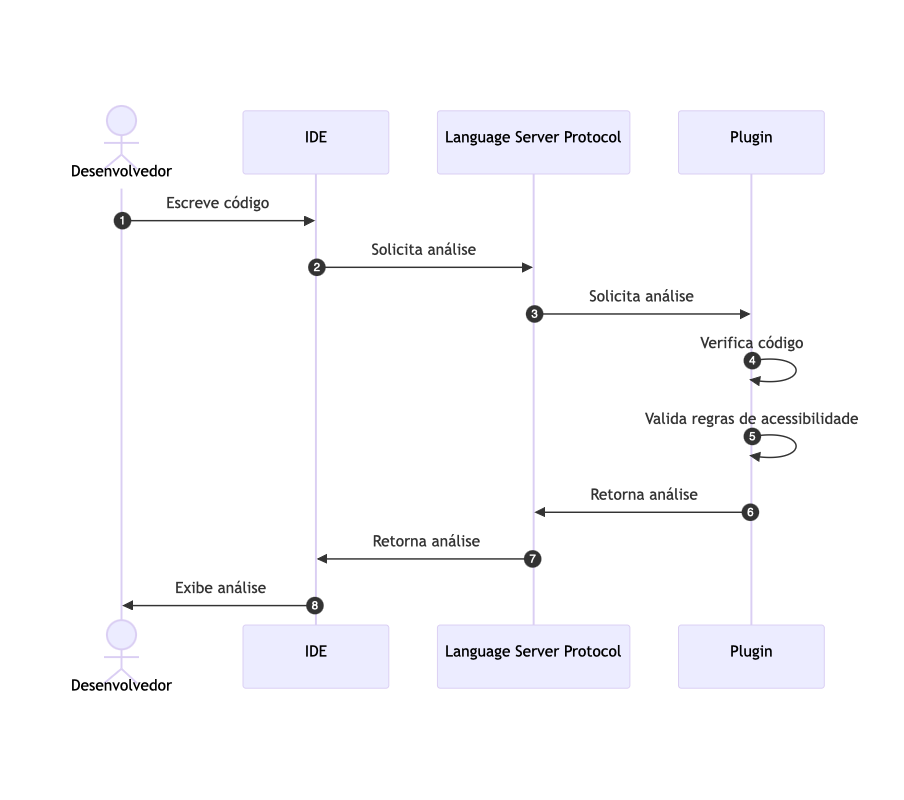
\includegraphics[width=325pt]{Assets/DiagramaSequenciaIDELSPPlugin.png}
	\fonte{\me{2024}}
\end{figure}

Como podemos ver na figura \ref{fig:diagrama-sequencia-plugin}, o desenvolvedor interage com o plugin através da IDE, que por sua vez executa a análise estática do código fonte da aplicação desenvolvida com Flutter. O plugin então marca o código fonte baseado nas regras de acessibilidade definidas e sugere correções automáticas. Isso torna todo o processo de desenvolvimento mais eficiente e permite que regras de acessibilidade sejam aplicadas desde o início do desenvolvimento sem a necessidade de compilar e executar a aplicação.

Entretanto o diagrama da figura \ref{fig:diagrama-sequencia-plugin} não mostra a interação do plugin com as regras de acessibilidade, para isso foi criado o diagrama de sequência da figura \ref{fig:diagrama-sequencia-regra-acessibilidade}:

\begin{figure}[!ht]
  \centering
  \caption{Interação do plugin com as regras de acessibilidade}\label{fig:diagrama-sequencia-regra-acessibilidade}
  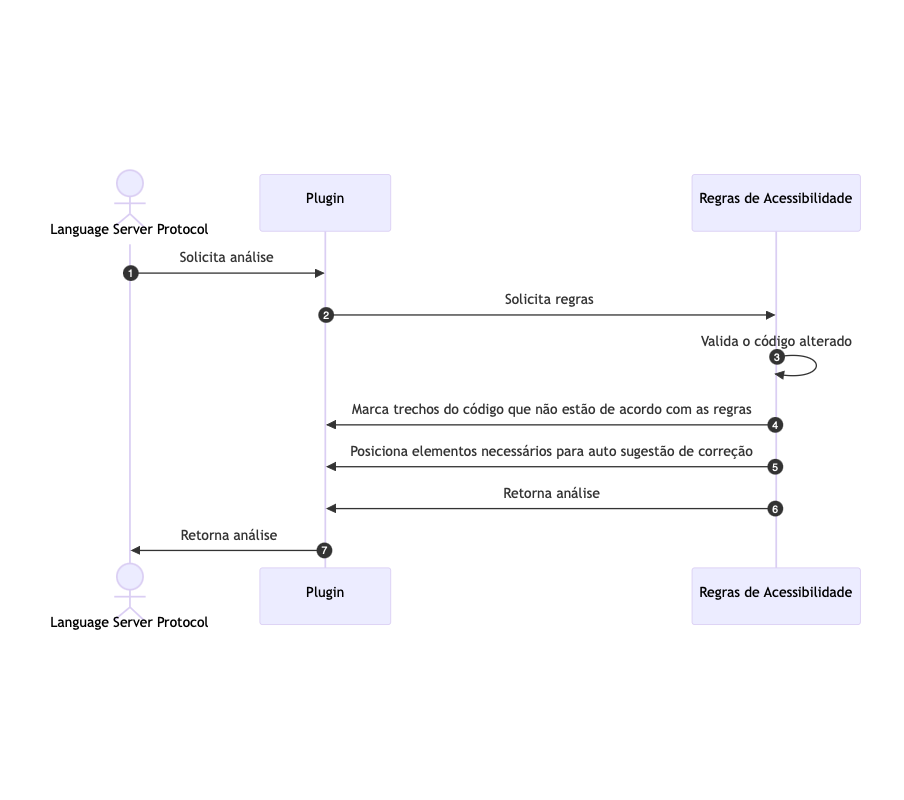
\includegraphics[width=325pt]{Assets/DiagramaPluginRegrasAcessibilidade.png}
  \fonte{\me{2024}}
\end{figure}

Como é possível identificar na figura \ref{fig:diagrama-sequencia-regra-acessibilidade}, o ponto de partida é o LSP que envia o código fonte do desenvolvedor para o Plugin, que então irá processar o código fonte aplicando todas as regras de acessibilidade definidas de uma forma sequencial. Cada regra de acessibilidade é aplicada ao código fonte e, caso uma inconsistência seja encontrada, o plugin marca o código fonte e sugere correções automáticas.

Um dos requisitos é ser possível utilizar o plugin através de uma linha de comando possibilitando integração com ambientes de integração contínua, para isso foi criado o diagrama de sequência da figura \ref{fig:diagrama-sequencia-linha-comando}:

\begin{figure}[!ht]
	\centering
	\caption{Interação do plugin com a linha de comando}\label{fig:diagrama-sequencia-linha-comando}
	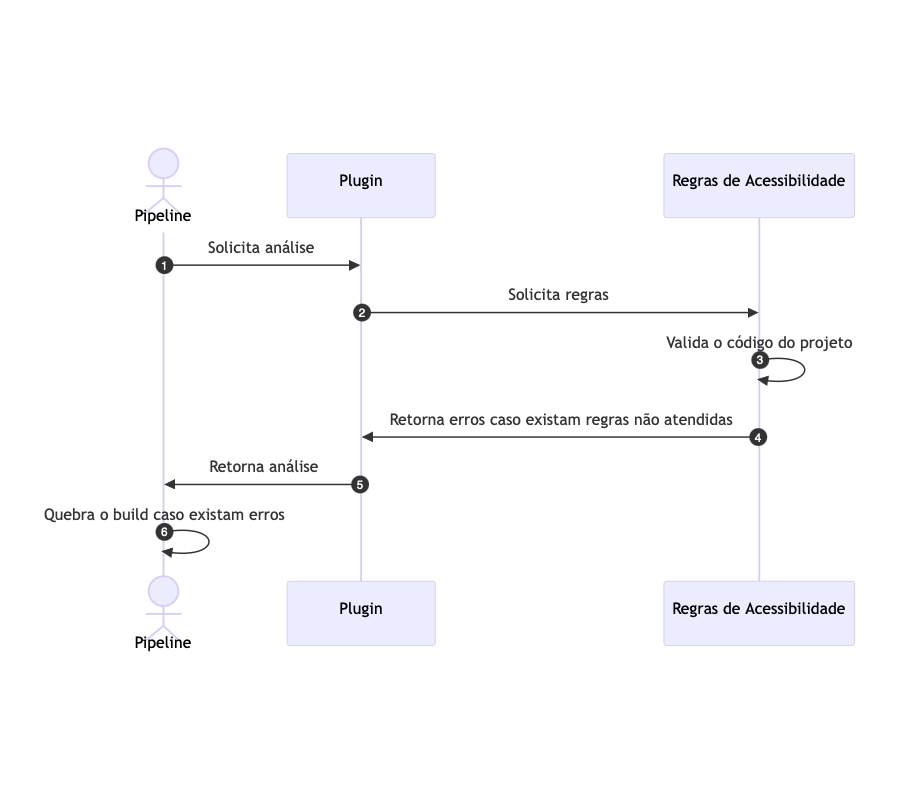
\includegraphics[width=325pt]{Assets/DiagramaSequenciaLinhaComando.png}
	\fonte{\me{2024}}
\end{figure}

O principal objetivo de integrar o plugin em ambientes de integração contínua é garantir que as regras de acessibilidade sejam aplicadas em todas as fases do desenvolvimento, desde a escrita do código até a compilação e execução da aplicação. Isso permite que os desenvolvedores travem a publicação de aplicações que não atendam aos requisitos de acessibilidade, garantindo que todas as aplicações desenvolvidas com Flutter sejam acessíveis a todos os usuários.

\subsection{Provas de Conceito}

\subsubsection{Extensão para Visual Studio Code}

Na concepção do projeto, a ideia era criar uma extensão para Visual Studio Code capaz de realizar a análise estática de código Dart e Flutter e retornar ao usuário as regras de acessibilidade que não foram seguidas. Porém, durante o desenvolvimento, percebeu-se que a seria necessário desenvolver toda uma infraestrutura de análise estática de código, o que demandaria muito tempo e recursos. Além disso, a equipe do Dart já provê uma API para análise estática de código, que será utilizada através do plugin \href{https://pub.dev/packages/analyzer}{analyzer}. 

Ademais, uma implementação focada em Visual Studio Code limitaria o alcance do projeto, uma vez que a extensão seria específica para essa IDE. Por isso, optou-se por desenvolver um plugin para LSP, que é uma interface de comunicação entre a IDE e o plugin, permitindo que o plugin seja utilizado em qualquer IDE que suporte LSP. Porém, ainda assim esbarra-se na necessidade de desenvolver uma infraestrutura de análise estática de código, o que demandaria muito tempo e recursos.

\subsubsection{Extensão para DevTools do Flutter}

DevTools é uma ferramenta de diagnóstico para Flutter que permite visualizar e inspecionar o comportamento da aplicação em execução. A ideia era criar uma extensão para DevTools capaz de realizar a análise estática de código Dart e Flutter e retornar ao usuário as regras de acessibilidade que não foram seguidas. Tal implementação seria agnóstica de IDE e uma vez que desenvolvida em Dart, poderia utilizar o pacote \href{https://pub.dev/packages/analyzer}{analyzer} para realizar a análise estática de código e processar o código fonte da aplicação desenvolvida com Flutter.

Porém, tal abordagem não seria capaz de marcar o código fonte da aplicação desenvolvida com Flutter, uma vez que DevTools é uma ferramenta de diagnóstico e não uma IDE. Sendo assim, tal ideia foi descartada após a realização de alguns testes.

\subsubsection{Plugin para Dart utilizando o pacote \href{https://pub.dev/packages/analyzer_plugin}{analyzer\_plugin}}

Haja vista que o projeto visava criar um plugin agnóstico de IDE porém ainda capaz de se comunicar com LSP tornando possível a marcação, sugestão de correção e validação de regras de acessibilidade, foi decidido utilizar o pacote \href{https://pub.dev/packages/analyzer_plugin}{analyzer\_plugin} para criar um plugin para Dart. O pacote \href{https://pub.dev/packages/analyzer_plugin}{analyzer\_plugin} é uma API para criar plugins para o Dart Analysis Server, que é uma ferramenta de análise estática de código Dart.

Seguindo a documentação oficial do pacote, foi então iniciado o desenvolvimento de uma prova de conceito. Para isso, foi então criado um novo projeto em Dart utilizando o template de pacote. Esse template estrutura um projeto Dart com uma base ideal para o desenvolvimento de um pacote que possa ser posteriormente publicado no repositório \href{https://pub.dev}{pub.dev}.

Para tal é necessário executar o seguinte comando: \texttt{dart create -t package-simple <nome\_do\_projeto>} que após a execução, irá gerar uma estrutura similar a apresentada na tabela \ref{tab:estrutura-projeto-dart}.

\begin{table}[!htbp]
	\centering
	\renewcommand{\arraystretch}{1.1}
	\caption{Estrutura de um projeto Dart utilizando o template de pacote}
	\label{tab:estrutura-projeto-dart}
	\ttfamily
	\begin{tabular}{ L{12cm} }
		\hline
		<nome\_do\_projeto> \\
		|--CHANGELOG.md \\
		|-- README.md \\
		|-- analysis\_options.yaml \\
		|-- example/ \\
		|---- <nome\_do\_projeto>\_example.dart \\
		|-- lib/ \\
		|---- <nome\_do\_projeto>.dart \\
		|---- src/ \\
		|------ <nome\_do\_projeto>\_base.dart \\
		|-- pubspec.lock \\
		|-- pubspec.yaml \\
		|-- test/ \\
		|---- <nome\_do\_projeto>\_test.dart \\
		\hline
	\end{tabular}
	\fontfamily{\rmdefault}\selectfont
	\vspace{2mm}
	\fonte{\me{2024}}
\end{table}

Com o projeto base criado, é então necessário adicionar as dependências necessárias para o desenvolvimento do plugin. Para isso, foi necessário executar o seguinte comando: \texttt{dart pub add analyzer\_plugin analyzer} que irá adicionar a dependência do pacote \href{https://pub.dev/packages/analyzer_plugin}{analyzer\_plugin} e do pacote \href{https://pub.dev/packages/analyzer}{analyzer} ao arquivo \texttt{pubspec.yaml}. Ambos são pacotes oficiais do time do Dart.

Seguindo então a documentação do \cite{documentacaoanalyzerplugin} foi possível chegar em uma implementação capaz de avaliar código fonte escrito em Dart e retornar as regras de acessibilidade que não foram seguidas. Entretanto a falta de suporte da equipe para com o pacote \href{https://pub.dev/packages/analyzer_plugin}{analyzer\_plugin} fez com que a implementação fosse abandonada. 

As principais dificuldades encontradas foram: 

\begin{itemize}
	\item Falta de documentação: A documentação oficial do pacote \href{https://pub.dev/packages/analyzer_plugin}{analyzer\_plugin} é escassa e não cobre todos os aspectos necessários para o desenvolvimento de um plugin para Dart.
	\item Falta de suporte: A equipe do Dart não fornece suporte para o pacote \href{https://pub.dev/packages/analyzer_plugin}{analyzer\_plugin}, o que torna difícil encontrar soluções para problemas específicos.
	\item Complexidade: O pacote \href{https://pub.dev/packages/analyzer_plugin}{analyzer\_plugin} é complexo e requer um conhecimento avançado de Dart e análise estática de código para ser utilizado corretamente.
	\item Falta de integração: O pacote não é capaz de integrar com o analisador padrão do Dart, o que dificulta a implementação de regras de acessibilidade personalizadas. Necessitando que o desenvolvedor que consuma o pacote tenha de executar uma série de comandos para que o plugin funcione corretamente.
\end{itemize}

\subsubsection{Plugin para Dart utilizando o pacote \href{https://pub.dev/packages/custom_lint_builder}{custom\_lint\_builder}}

Após a tentativa frustrada de utilizar o pacote \href{https://pub.dev/packages/analyzer_plugin}{analyzer\_plugin}, foi então decidido utilizar o pacote \href{https://pub.dev/packages/custom_lint_builder}{custom\_lint\_builder} para criar um plugin para Dart. Apesar de ele necessitar que o usuário final importe o pacote \href{https://pub.dev/packages/custom_lint}{custom\_lint} no seu projeto, utilize arquivos diferentes para a personalização de regras de acessibilidade, e também necessitar de uma interface de linha de comando própria, sendo incompatível com o comando \texttt{dart analyze} do Dart, ele é atualmente a melhor opção para a criação de um plugin "linter" para Dart. Porém ele ainda possuí um problema que não é simples de resolver sem envolver o time de desenvolvimento do Dart, ele não é capaz de integrar com comandos como \texttt{dart analyze} e \texttt{dart format}. Entretanto, não existe alternativa viável para a criação de um plugin "linter" para Dart que atenda esse requisito. 

Tal pacote se mostrou mais simples de utilizar e mais bem documentado que o pacote \href{https://pub.dev/packages/analyzer_plugin}{analyzer\_plugin}. Além disso, ele é capaz de integrar com o analisador padrão do Dart, o que facilita a implementação de regras de acessibilidade personalizadas. 

Para executar em um ambiente de integrado contínua, basta executar o comando \texttt{dart run custom\_lint} que irá analisar o código fonte do projeto e retornar as regras de acessibilidade que não foram seguidas, com um comportamento similar ao comando \texttt{dart analyze} do Dart.

\section{Mapeamento Sistemático da Literatura}\label{sec:msl}

Com a conclusão da etapa de Modelagem e provas de conceito, a próxima etapa é o Mapeamento Sistemático da Literatura, onde serão identificadas as regras de acessibilidade mais utilizadas e criado um conjunto de regras de acessibilidade padrão.

\subsection{Protocolo de Pesquisa}

Como protocolo de pesquisa para a realização do Mapeamento Sistemático da Literatura, foi utilizado o descrito no apêndice 1 do relatório técnico de \cite{srufrj}. A partir dele, as etapas serão condensadas em: Definição do Problema, Questões de Pesquisa, Seleção de Bases de Dados, Critérios de Inclusão e Exclusão, Seleção de Estudos e Síntese dos Dados.

\subsubsection{Questões de Pesquisa}

\begin{itemize}
	\item QP1: Quais são as regras de acessibilidade mais utilizadas em móveis?
	\item QP2: Existe um conjunto de regras de acessibilidade padrão para aplicações móveis?
	\item QP3: Como as regras de acessibilidade são aplicadas em aplicações móveis?
\end{itemize}

\subsubsection{Seleção de Bases de Dados}

Para o levantamento de dados de uma forma mais automatizada através da utilização de ferramentas de busca com suporte a consultas estruturadas, foi decidido utilizar as seguintes bases de dados:

\begin{itemize}
	\item \href{https://ieeexplore.ieee.org/}{IEEE Xplore}
	\item \href{https://dl.acm.org/}{ACM Digital Library}
	\item \href{https://scholar.google.com/}{Google Scholar}
\end{itemize}

Como \texttt{string} de busca após algumas iterações para melhor ajuste, foi definida a presente na tabela \ref{tab:strings-de-busca}. Ela foi utilizada para realizar a busca nas bases de dados selecionadas.

\begin{table}[!htbp]
	\centering
	\renewcommand{\arraystretch}{1.1}
	\caption{Strings de busca}
	\label{tab:strings-de-busca}
	\begin{tabular}{ L{12cm} }
		\hline
		("mobile development" OR "mobile app*") AND ("accessibility" OR "accessible design" OR "inclusive design" OR "digital inclusion") AND ("tool*" OR "guidelines" OR "legislation" OR "legal" OR "requirements" OR "compliance" OR "challenges" OR "demand") AND NOT("W3C" OR "web") \\
		\hline
	\end{tabular}
	\vspace{2mm}
	\fonte{\me{2023}}
\end{table}

Foi utilizado a lingua inglesa para a busca, uma vez que a maioria dos artigos científicos estão escritos nessa língua. Além disso, foi definido o período de 2010 a 2023 para a busca, uma vez que a acessibilidade em aplicações móveis é um tema relativamente novo e a maioria dos artigos científicos sobre o assunto foram publicados nesse período.

\subsubsection{Critérios de Inclusão e Exclusão}

Os critérios de inclusão e exclusão foram definidos para garantir que apenas os artigos relevantes para o tema da pesquisa fossem selecionados. Os critérios de inclusão e exclusão são apresentados na tabela \ref{tab:criterios-inclusao-exclusao}.

\begin{table}[!htbp]
	\centering
	\renewcommand{\arraystretch}{1.1}
	\caption{Critérios de inclusão e exclusão}
	\label{tab:criterios-inclusao-exclusao}
	\begin{tabular}{ L{12cm} }
		\hline
		Critérios de Inclusão \\
		\hline
		Artigos que abordam o tema da acessibilidade em aplicações móveis \\
		Artigos publicados entre 2010 e 2023 \\
		Artigos escritos em inglês \\
		Artigos disponíveis gratuitamente \\
		Regras de acessibilidade aplicáveis em aplicações móveis \\
		\hline
		Critérios de Exclusão \\
		\hline
		Artigos que não abordam o tema da acessibilidade em aplicações móveis \\
		Artigos publicados antes de 2010 ou após 2023 \\
		Artigos escritos em outro idioma que não o inglês \\
		Regras de acessibilidade não aplicáveis em aplicações móveis \\
		\hline
	\end{tabular}
	\vspace{2mm}
	\fonte{\me{2023}}
\end{table}

\subsubsection{Seleção de Estudos}

Com as bases de dados selecionadas e os critérios de inclusão e exclusão definidos, foi possível realizar a busca e selecionar os estudos relevantes para a pesquisa. A busca foi realizada utilizando a \texttt{string} de busca definida anteriormente na tabela \ref{tab:strings-de-busca} e os critérios de inclusão e exclusão definidos na tabela \ref{tab:criterios-inclusao-exclusao}.

Os resultados da busca obtidos estão destacados na tabela \ref{tab:quantidade-de-estudos}.

\begin{table}[!htbp]
	\centering
	\renewcommand{\arraystretch}{1.1}
	\caption{Quantidade de estudos encontrados}
	\label{tab:quantidade-de-estudos}
	\begin{tabular}{ L{4cm}  L{2cm}  L{2cm}  L{2cm}  L{3cm} }
		\hline
		Base de Dados & Total de Estudos & Estudos Incluídos & Estudos Excluídos & Estudos Selecionados \\
		\hline
		IEEE Xplore & 247 & 17 & 230 & 2 \\
		ACM Digital Library & 32 & 12 & 20 & 3 \\
		Google Scholar & 17700 & 7 & 17693 & 2 \\
		\hline
	\end{tabular}
	\vspace{2mm}
	\fonte{\me{2024}}
\end{table}

\subsubsection{Síntese dos Dados}\label{sec:sintese-dados}

Com os trabalhos selecionados, foi possível identificar um conjunto comum de regras de acessibilidade juntamente as definidas pelas plataformas Apple \cite{iosaccessibility} e Google \cite{androidaccessibility}. As regras de acessibilidade identificadas estão apresentadas na tabela \ref{tab:regras-acessibilidade}.

Porém um fato importante a ser destacado é que a maioria dos artigos relevantes para a pesquisa não estavam disponíveis gratuitamente, o que dificultou a realização do Mapeamento Sistemático da Literatura. Além disso, a falta de acesso a artigos científicos relevantes para a pesquisa fez com que não fosse possível identificar um conjunto de regras de acessibilidade padrão para aplicações móveis. Isso pode ser fruto da \texttt{string} de busca utilizada, que pode não ter sido a mais adequada para a pesquisa.

\section{Regras de Acessibilidade}\label{sec:regras-acessibilidade}

Seguindo a documentação oficial da Apple \cite[p. ~312]{iosaccessibility}, Google \cite{androidaccessibility} e dos trabalhos selecionados na seção \ref{sec:sintese-dados} do Mapeamento Sistemático da Literatura realizado, foi possível identificar um conjunto de regras de acessibilidade que são comuns a ambas as plataformas. Essas regras de acessibilidade serão utilizadas como base para a criação de um conjunto de regras de acessibilidade padrão para aplicações móveis desenvolvidas com Flutter. Podemos visualizar ela na tabela \ref{tab:regras-acessibilidade}.

O trabalho realizado por \cite{studyofaccessibilityguidelinesofmobileapplications} levantou quais as principais violações de acessibilidade em um conjunto de aplicativos selecionados para testes, e nele é possível identificar houveram 25 violações da regra de falta de texto alternativo para imagens e 29 violações da regra de falta de rótulos descritivos para elementos interativos. Para tal, a regra de acessibilidade \ref{ra:tooltip} e \ref{ra:descricao-imagens} foram escolhidas para serem implementadas no projeto tornando assim, um requisito aplicações móveis desenvolvidas com Flutter possuírem uma descrição alternativa para imagens e rótulos descritivos para elementos interativos.

\newcounter{ra} 
\renewcommand{\thera}{RA\arabic{ra}}

\begin{table}[!htbp]
	\centering
	\renewcommand{\arraystretch}{1.1}
	\caption{Regras de acessibilidade baseadas nas recomendações de ambas as plataformas}
	\label{tab:regras-acessibilidade}
	\begin{tabular}{ R{2.5cm}  L{12cm} }
		\hline
		Regra de Acessibilidade & Descrição \\
		\hline
		\refstepcounter{ra}\thera\label{ra:tooltip} & Utilize rótulos descritivos para todos os elementos interativos \\
		\refstepcounter{ra}\thera\label{ra:descricao-imagens} & Forneça descrições de texto alternativas para imagens \\
		\refstepcounter{ra}\thera\label{ra:feedback-visual} & Forneça feedback visual, auditivo ou tátil para todas as interações do usuário \\
		\refstepcounter{ra}\thera\label{ra:largura-minima} & Elementos interativos devem possuir um mínimo de 48pt de largura e altura \\
		\refstepcounter{ra}\thera\label{ra:contraste-minimo} & Forneça um contraste mínimo de 4.5:1 entre o texto e o plano de fundo \\
		\hline
	\end{tabular}
	\vspace{2mm}
	\fonte{\me{2024}}
\end{table}

Para a regra de acessibilidade \ref{ra:feedback-visual}, foi utilizado como base além das documentações oficiais das plataformas o trabalho de \cite[p. 6]{accessibilityinmobileapplicationsforelderyusers} identificou a dificuldade de pessoas idosas em perceber interações em aplicações móveis, e que a falta de feedback visual, auditivo ou tátil para interações do usuário é uma das principais barreiras de acessibilidade para esse público. Com base nisso, foi definido que a regra de acessibilidade \ref{ra:feedback-visual} deve ser seguida por todas as aplicações móveis desenvolvidas com Flutter.

Ademais, \cite{accessibilityinmobileapplicationsforelderyusers} e \cite{studyofaccessibilityguidelinesofmobileapplications} identificaram que a falta de contraste entre o texto e o plano de fundo é uma das principais barreiras de acessibilidade em aplicações móveis, contribuindo com a escolha da regra de acessibilidade \ref{ra:contraste-minimo}. 

Tais regras de acessibilidade serão utilizadas como base para a criação de um conjunto de regras de acessibilidade padrão para aplicações móveis desenvolvidas com Flutter. Elas serão aplicadas ao código fonte da aplicação desenvolvida com Flutter e o plugin irá marcar o código fonte e sugerir correções automáticas caso uma inconsistência seja encontrada.

\section{Projeto}

Com a conclusão da etapa de Mapeamento Sistemático da Literatura, a próxima etapa é o Projeto, onde será projetada a arquitetura de integração com o Flutter e selecionados os frameworks, bibliotecas e linguagens que serão usados no desenvolvimento da ferramenta.

\subsection{Arquitetura de Integração com o Flutter}

A arquitetura de integração com o Flutter foi projetada para ser simples e eficiente, permitindo que o plugin seja utilizado em qualquer IDE que suporte LSP. A arquitetura é composta por três componentes principais: o LSP, o Plugin e o Dart Analysis Server.

Como descrito na seção de Provas de Conceito, foi escolhido o pacote \href{https://pub.dev/packages/custom_lint_builder}{custom\_lint\_builder} para criar um plugin para Dart.

Seguindo sua documentação \cite{customlintbuilder}, foi possível criar uma estrutura de diretórios e arquivos que permite a criação de regras de acessibilidade personalizadas e a integração com o analisador padrão do Dart. Ela está disposta na tabela  \ref{tab:estrutura-diretorios-arquivos}.

Uma regra de \texttt{lint} utilizando o pacote usualmente necessita de uma classe que estende \texttt{LintRule} e sobrescreve o método \texttt{register} para registrar a regra de acessibilidade. Ademais, podemos definir regras de correção automática criando uma nova classe que estende \texttt{DartFix}. Mais detalhes sobre como implementar serão descritos na próxima seção com um exemplo prático com uma das regras de acessibilidade implementadas.

\begin{table}[!htbp]
	\centering
	\renewcommand{\arraystretch}{1.1}
	\caption{Estrutura de diretórios e arquivos do projeto}
	\label{tab:estrutura-diretorios-arquivos}
	\ttfamily
	\begin{tabular}{ L{12cm} }
		\hline
		<projeto> \\
		|-- analysis\_options.yaml \\
		|-- lib/ \\
		|---- <nome\_do\_projeto>.dart \\
		|---- rules/ \\
		|------ <nome\_da\_regra>/ \\
		|-------- <nome\_da\_regra>\_rule.dart \\
		|-------- <nome\_da\_regra>\_fix.dart \\
		|-- pubspec.yaml \\
		\hline
	\end{tabular}
	\fontfamily{\rmdefault}\selectfont
	\vspace{2mm}
	\fonte{\me{2024}}
\end{table}

Com a estrutura da tabela \ref{tab:estrutura-diretorios-arquivos}, é possível escalar de forma simples e eficiente a criação de regras de acessibilidade personalizadas e a integração com o analisador do pacote \href{https://pub.dev/packages/custom_lint}{custom\_lint}. Pode ser resumido a criação de uma nova pasta dentro de \texttt{rules} com o nome da regra de acessibilidade.

O principal objetivo é permitir que outros desenvolvedores possam ampliar o conjunto de regras de acessibilidade padrão para aplicações móveis desenvolvidas com Flutter, garantindo que todas as aplicações desenvolvidas com Flutter sejam acessíveis a todos os usuários.

\section{Desenvolvendo uma Regra de Acessibilidade}

Para exemplificar como desenvolver uma regra de acessibilidade utilizando o pacote \href{https://pub.dev/packages/custom_lint}{custom\_lint}, foi escolhida a regra de acessibilidade \ref{ra:tooltip}: Utilize rótulos descritivos para todos os elementos interativos. Essa regra de acessibilidade é comum a ambas as plataformas e é uma das regras de acessibilidade mais utilizadas em aplicações móveis.

No Flutter, seguindo sua documentação oficial \cite{flutter} podemos notar que em elementos como o \texttt{IconButton} é possível adicionar um \texttt{tooltip} que é exibido quando o usuário passa o mouse sobre o elemento. Esse \texttt{tooltip} é um rótulo descritivo que descreve a função do elemento interativo.

O objetivo final está disposto na figura \ref{fig:exemplo-codigo-fonte-tooltip} onde é possível visualizar que a IDE marca o código fonte e sugere correções automáticas quando um \texttt{IconButton} não possui um \texttt{tooltip}.

\begin{figure}[!ht]
	\centering
	\caption{Exemplo de código fonte com a regra de acessibilidade \ref{ra:tooltip} não seguida com a IDE marcando o código fonte}\label{fig:exemplo-codigo-fonte-tooltip}
	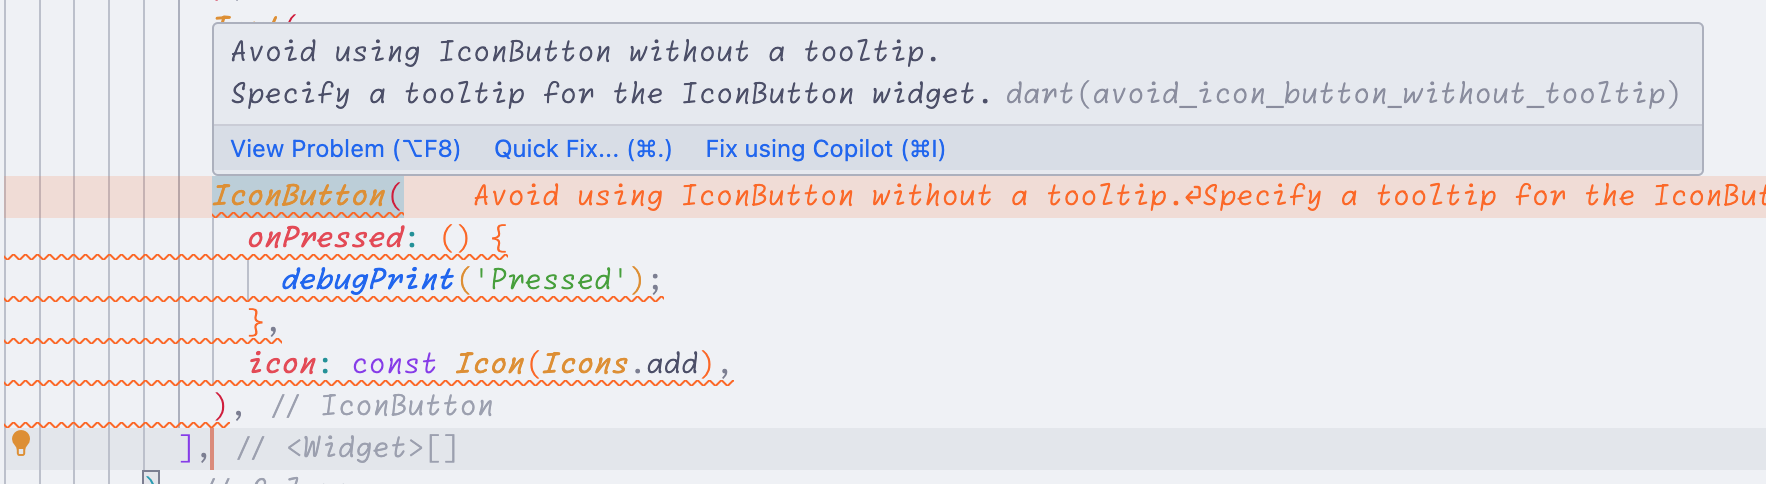
\includegraphics[width=425pt]{Assets/PrintIDEAviso.png}
	\fonte{\me{2024}}
\end{figure}

Também podemos visualizar na figura \ref{fig:exemplo-correcao-automatica-tooltip} que a IDE sugere correções automáticas para a regra de acessibilidade \ref{ra:tooltip}. E ao aceitar a correção automática, o \texttt{tooltip} é adicionado ao \texttt{IconButton} bastando o desenvolvedor adicionar o texto da descrição do elemento interativo.

\begin{figure}[!ht]
	\centering
	\caption{Exemplo de correção automática para a regra de acessibilidade \ref{ra:tooltip}}\label{fig:exemplo-correcao-automatica-tooltip}
	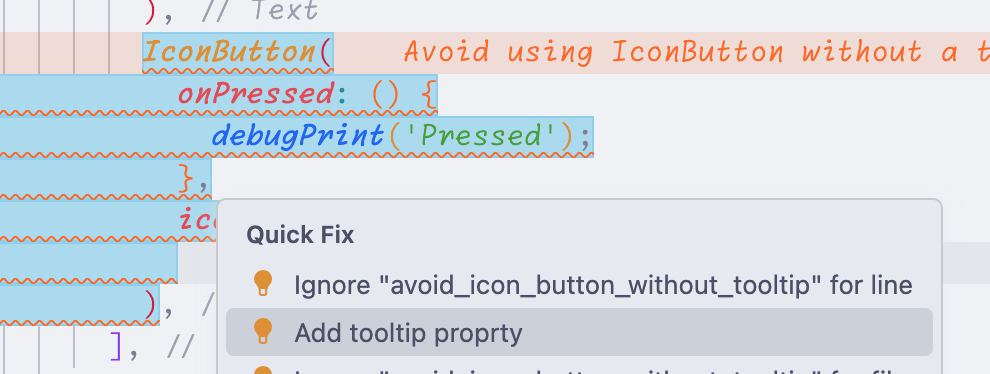
\includegraphics[width=425pt]{Assets/PrintIDECorrecao.png}
	\fonte{\me{2024}}
\end{figure}

Também visando a possibilidade de utilização em ambientes de integração continua, na figura \ref{fig:exmplo-comando-erro} é possível visualizar a execução do comando \seqsplit{dart run custom\_lint} que analisa o código fonte do projeto e retorna as regras de acessibilidade que não foram seguidas.

\begin{figure}[!ht]
	\centering
	\caption{Exemplo da execução do comando \texttt{dart run custom\_lint}}\label{fig:exmplo-comando-erro}
	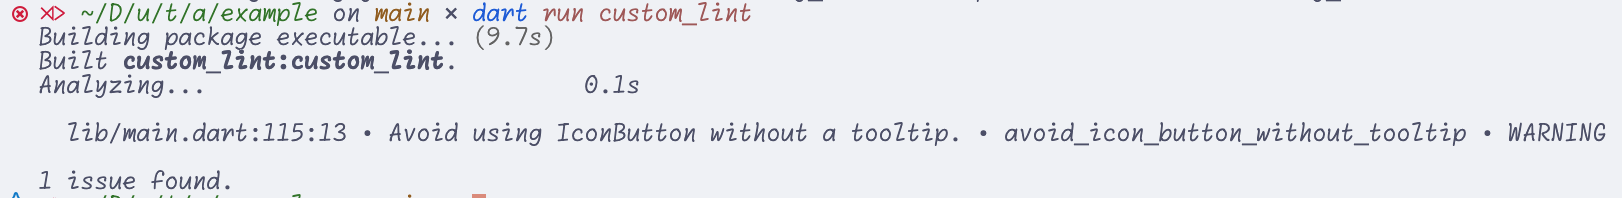
\includegraphics[width=425pt]{Assets/PrintComandoCustomLint.png}
	\fonte{\me{2024}}
\end{figure}

Dessa forma é possível garantir que sempre que um desenvolvedor adicione um \seqsplit{IconButton} em sua aplicação desenvolvida com Flutter, ele seja obrigado a adicionar um \seqsplit{tooltip} que descreva a função do elemento interativo, tornando a aplicação mais acessível a todos os usuários.

\subsection{Estruturando o Projeto}

Para implementar a regra de acessibilidade \ref{ra:tooltip}: Utilize rótulos descritivos para todos os elementos interativos, foi criada a seguinte estrutura de diretórios e arquivos:

\begin{table}[!htbp]
	\centering
	\renewcommand{\arraystretch}{1.1}
	\caption{Estrutura de diretórios e arquivos para a regra de acessibilidade \ref{ra:tooltip}}
	\label{tab:estrutura-diretorios-arquivos-ra1}
	\ttfamily
	\begin{tabular}{ L{12cm} }
		\hline
		accessibility\_lint \\
		|-- analysis\_options.yaml \\
		|-- lib/ \\
		|---- accessibility\_lint.dart \\
		|---- rules/ \\
		|------ avoid\_icon\_button\_without\_tooltip\_rule/ \\
		|-------- avoid\_icon\_button\_without\_tooltip\_rule\_rule.dart \\
		|-------- avoid\_icon\_button\_without\_tooltip\_rule\_fix.dart \\
		|-- pubspec.yaml \\
		\hline
	\end{tabular}
	\fontfamily{\rmdefault}\selectfont
	\vspace{2mm}
	\fonte{\me{2024}}
\end{table}

Com a estrutura da tabela \ref{tab:estrutura-diretorios-arquivos-ra1} pronta, podemos partir para a implementação de tal regra. 
Com a estrutura definida, precisamos alterar o arquivo inicial do projeto \seqsplit{accessibility\_lint.dart} para registrar a regra de acessibilidade e verificar se um \texttt{IconButton} possui um \texttt{tooltip}. A figura \ref{fig:accessibility-lint} apresenta o código fonte.

\begin{figure}[!htbp]
\centering
\caption{Código fonte do arquivo accessibility\_lint.dart}\label{fig:accessibility-lint}
\begin{lstlisting}
import 'package:custom_lint_builder/custom_lint_builder.dart';

import 'src/rules/avoid_icon_button_without_tooltip/....dart';

PluginBase createPlugin() => _AccessibilityLintPlugin();

class _AccessibilityLintPlugin extends PluginBase {
	@override
	List<LintRule> getLintRules(
		final CustomLintConfigs configs,
	) =>
			<LintRule>[
				const AvoidIconButtonWithoutTooltipRule(),
			];
}		
\end{lstlisting}
\vspace{2mm}
\fonte{\me{2024}}
\end{figure}

Para criar um plugin para o pacote \href{https://pub.dev/packages/custom_lint}{custom\_lint}, é necessário criar uma classe que estende \texttt{PluginBase} e sobrescrever o método \texttt{getLintRules} para retornar uma lista de regras de acessibilidade. Na linha 5 da figura \ref{fig:accessibility-lint}, é definido um método \texttt{createPlugin} que retorna uma instância da classe \texttt{\_AccessibilityLintPlugin}. Na linha 9 sobrescrevemos o método \texttt{getLintRules} para retornar uma lista de regras de acessibilidade, que no caso é a regra de acessibilidade \seqsplit{AvoidIconButtonWithoutTooltipRule} que será implementada na próxima seção.

\subsection{Implementando a Regra de Acessibilidade}

Para implementar a regra de acessibilidade, iremos primeiro alterar o arquivo \seqsplit{avoid\_icon\_button\_without\_tooltip\_rule\_rule.dart} para registrar a regra de acessibilidade e verificar se um \texttt{IconButton} possui um \texttt{tooltip}. A figura \ref{fig:avoid-icon-button-without-tooltip-rule} apresenta o código fonte. Em seguida será destacado cada passo da implementação para melhor compreensão.

Para criar uma regra de \texttt{lint} utilizando o pacote \href{https://pub.dev/packages/custom_lint}{custom\_lint}, é criar uma estender a classe \texttt{DartLintRule}, assim como é possível visualizar na linha 7 da figura \ref{fig:avoid-icon-button-without-tooltip-rule}. Também é necessário sobrescrever o método \texttt{run} para registrar a regra de acessibilidade e tornar visível para o pacote.

Nas linhas 10 a 14 da figura \ref{fig:avoid-icon-button-without-tooltip-rule}, é definido os textos que irão retornar ao usuário caso a regra de acessibilidade não seja seguida. Ela é um objeto da class e \texttt{LintCode} que recebe o nome da regra, a mensagem de problema e a mensagem de correção. Nela definimos na linha 11 que o nome da regra é "\seqsplit{avoid\_icon\_button\_without\_tooltip}", na linha 12 a mensagem de problema é "\texttt{Avoid using IconButton without a tooltip.}", na linha 13 a mensagem de correção é "\texttt{Specify a tooltip for the IconButton widget.}" e por fim na linha 14 definimos o nível de severidade do erro como \texttt{WARNING} pois a regra de acessibilidade não é um erro de compilação.

Com essa definição básica especificada, agora precisamos efetivamente construir o código que irá fazer a validação de tal regra \cite{customlintbuilder}. Usualmente, aplicações em Flutter, possuem um esquema de definição declarativa de interface no qual as propriedades de um "Widget" são passadas como argumentos para o construtor do mesmo.

\begin{figure}[!htbp]
\centering
\caption{Código fonte do arquivo avoid\_icon\_button\_without\_tooltip\_rule.dart}\label{fig:avoid-icon-button-without-tooltip-rule}
\begin{lstlisting}
import 'package:analyzer_dart/ast/ast.dart';
import 'package:analyzer/error/listener.dart';
import 'package:custom_lint_builder/custom_lint_builder.dart';

import 'avoid_icon_button_without_tooltip_fix.dart';

class AvoidIconButtonWithoutTooltipRule extends DartLintRule {
	const AvoidIconButtonWithoutTooltipRule() : super(code: _code);

	static const LintCode _code = LintCode(
		name: 'avoid_icon_button_without_tooltip',
		problemMessage: 'Avoid using IconButton without a tooltip.',
		correctionMessage: 'Specify a tooltip for the IconButton widget.',
		errorSeverity: ErrorSeverity.WARNING,
	);

	@override
	void run(
		final CustomLintResolver resolver,
		final ErrorReporter reporter,
		final CustomLintContext context,
	) {
		context.registry.addInstanceCreationExpression((
			final InstanceCreationExpression node,
		) {
			final String constructorName = node.constructorName.type.toString();

			if (constructorName != 'IconButton') return;

			bool hasTooltip = false;
      for (final Expression argument in node.argumentList.arguments) {
        if (argument is! NamedExpression) continue;
        final String name = argument.name.label.name;

        if (name != 'tooltip') continue;

        hasTooltip = true;
        break;
      }

      if (hasTooltip) return;

      reporter.atNode(node, _code);
		});
	}

	@override
	List<Fix> getFixes() => <Fix>[AvoidIconButtonWithoutTooltipFix()];
}
\end{lstlisting}
\vspace{2mm}
\fonte{\me{2024}}
\end{figure}

Para verificar se um \texttt{IconButton} possui um \texttt{tooltip}, é necessário verificar se o construtor do \texttt{IconButton} possui um argumento chamado \texttt{tooltip}. Para isso, é necessário percorrer a lista de argumentos do construtor e verificar se existe um argumento chamado \texttt{tooltip}. Uma vez que o pacote \href{https://pub.dev/packages/custom_lint}{custom\_lint} não fornece uma maneira de acessar o código fonte do construtor, é necessário utilizar a API do pacote \href{https://pub.dev/packages/analyzer}{analyzer}. Ela fornece uma árvore de sintaxe abstrata \cite{compiladores} que representa o código fonte do arquivo analisado e permite acessar os elementos do código fonte, como construtores, argumentos e propriedades.

O primeiro passo é realizado na linha 25, onde definimos uma variável \seqsplit{constructorName} que recebe o nome do construtor do nó da árvore que está sendo visitado naquele momento. Para facilitar a compreensão de como a árvore é construída, é possível visualizar a figura \ref{fig:flutter-component-tree}.

\begin{figure}[!htbp]
	\centering
	\caption{Árvore de componentes de um código fonte Dart}
	\label{fig:flutter-component-tree}
	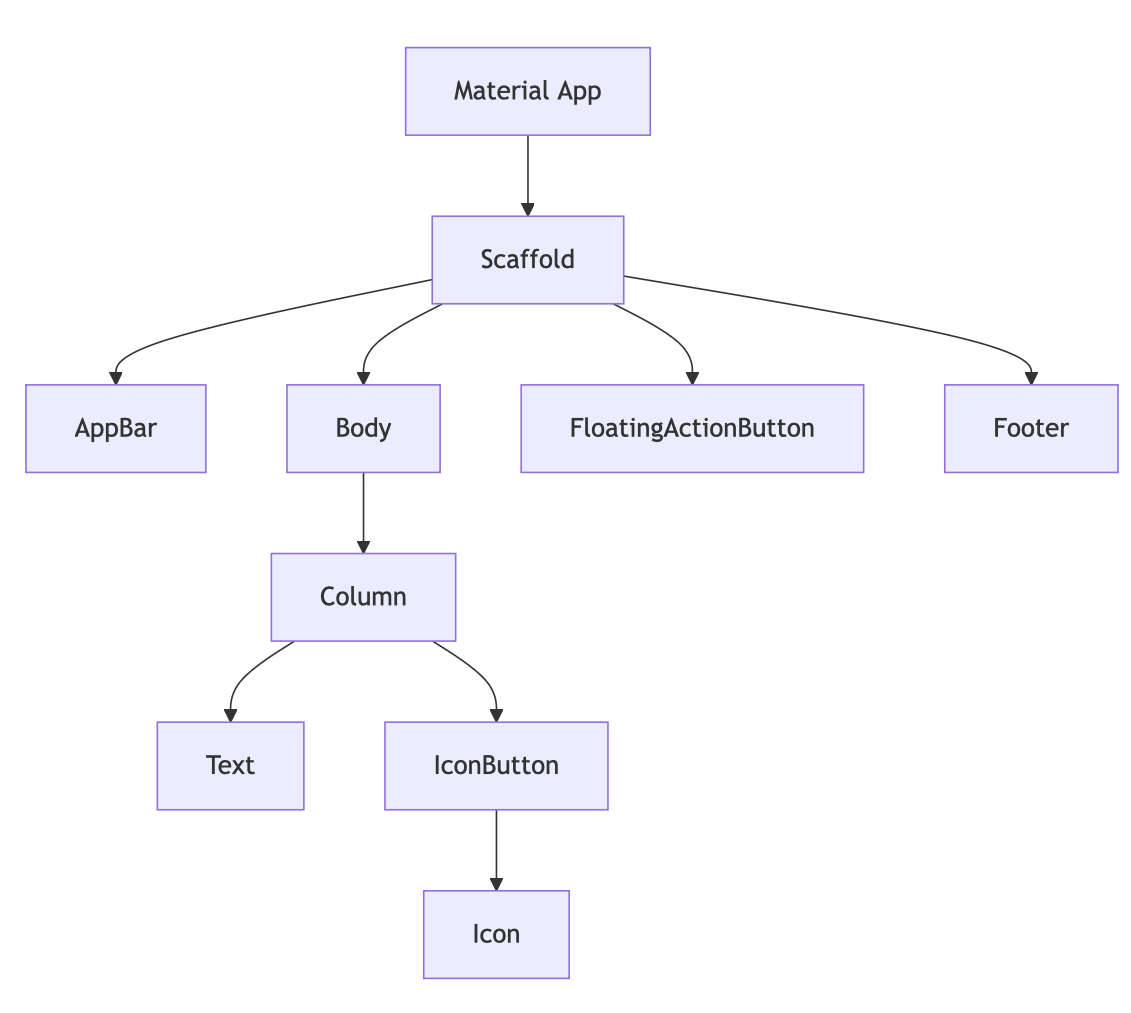
\includegraphics[width=325pt]{Assets/FlutterComponentTree.png}
	\fonte{\me{2024}}
\end{figure}

Uma vez que estamos apenas interessados no construtor do \texttt{IconButton}, é necessário verificar se o nome do construtor é igual a \texttt{IconButton}. Isso é feito na linha 27, onde verificamos se o nome do construtor é diferente de \texttt{IconButton}. Caso não seja, a regra de acessibilidade não é aplicada e a execução já retorna na mesma linha.

Com a certeza de que o nó é um \texttt{IconButton}, agora é necessário verificar se ele já possui o atributo \texttt{tooltip} conforme definido na documentação do Flutter \cite{flutter}. Para isso, é necessário percorrer a lista de argumentos do construtor e verificar se o argumento está sendo utilizado. Com isso, na linha 30 é iniciado um laço de repetição que percorre a lista de argumentos do construtor. Tais argumentos possuem o tipo \texttt{Expression} e é necessário verificar se ele é um \texttt{NamedExpression} que é um argumento nomeado. Caso não seja, a execução retorna na linha 31. Se o nome desse argumento nomeado não for \texttt{tooltip}, a execução retorna na linha 33. Caso contrário, a variável \texttt{hasTooltip} é definida como verdadeira e a execução do laço de repetição se encerra.

Haja vista que a regra de acessibilidade é aplicada apenas quando um \texttt{IconButton} não possui um \texttt{tooltip}, é necessário verificar o estado da variável \texttt{hasTooltip}. Em caso de estar definida como verdadeira, a execução retorna na linha 35. Caso contrário, a regra de acessibilidade é aplicada e a mensagem de problema é reportada na linha 37.

Com isso, temos a primeira regra de acessibilidade implementada. A próxima etapa é implementar a regra de correção automática que irá sugerir a adição de um \texttt{tooltip} para o \texttt{IconButton}.

\subsection{Implementando a Correção Automática}

Para implementar a regra de correção automática, iremos alterar o arquivo \seqsplit{avoid\_icon\_button\_without\_tooltip\_rule\_fix.dart} para sugerir a adição de um \texttt{tooltip} para o \texttt{IconButton}. A figura \ref{fig:avoid-icon-button-without-tooltip-rule-fix} apresenta o código fonte.

\begin{figure}[!htbp]
\centering
\caption{Código fonte do arquivo avoid\_icon\_button\_without\_tooltip\_fix.dart}\label{fig:avoid-icon-button-without-tooltip-rule-fix}
\begin{lstlisting}
class AvoidIconButtonWithoutTooltipFix extends DartFix {
	@override
	void run(
		final CustomLintResolver resolver,
		final ChangeReporter reporter,
		final CustomLintContext context,
		final AnalysisError analysisError,
		final List<AnalysisError> others,
	) {
		context.registry.addInstanceCreationExpression(
			(final InstanceCreationExpression node) {
				if (!analysisError.sourceRange.intersects(node.sourceRange)) {
					return;
				}

				final String constructorName = node.constructorName.type.toString();
				if (constructorName != 'IconButton') return;

				bool haveCommaBeforeEndToken = false;
				if (node.endToken.previous?.lexeme == ',') {
					haveCommaBeforeEndToken = true;
				}

				reporter
					.createChangeBuilder(
						message: 'Add tooltip property',
						priority: 0,
					).addDartFileEdit((
						final DartFileEditBuilder builder,
					) {
						final int offset = node.endToken.offset - 1;

						builder.addInsertion(
							offset,
							(final DartEditBuilder builder) {
								if (haveCommaBeforeEndToken) {
									builder.write(" tooltip: '");
								} else {
									builder.write(", tooltip: '");
								}

								builder..selectHere()..writeln("',");
							},
						);
					},
				);
			},
		);
	}
}
\end{lstlisting}
\vspace{2mm}
\fonte{\me{2024}}
\end{figure}

Assim como na figura \ref{fig:avoid-icon-button-without-tooltip-rule}, a etapa inicial, seguindo a documentação \cite{customlintbuilder} é estender uma classe do pacote utilizado na criação do plugin. Nesse caso, é a classe \texttt{DartFix} que é utilizada para implementar regras de correção automática. Na linha 1 da figura \ref{fig:avoid-icon-button-without-tooltip-rule-fix}, é definida a classe \seqsplit{AvoidIconButtonWithoutTooltipFix} que estende a classe \texttt{DartFix}. O único método que precisa ser implementado é o método \texttt{run} que é chamado quando a regra de acessibilidade é violada.

A etapa inicial, como definida na na linha 12, é verificar se o erro de análise está contido no nó da árvore que está sendo visitado. Caso não esteja, a execução retorna na linha 13. Em seguida, é verificado se o nó é um \texttt{IconButton} na linha 16. Caso não seja, a execução retorna na linha 17.

Uma vez que o nó é um \texttt{IconButton}, é necessário verificar se o último token do nó é uma vírgula. Isso é necessário para garantir que a correção automática seja aplicada corretamente. Caso o último token do nó seja uma vírgula, a variável \texttt{haveCommaBeforeEndToken} é definida como verdadeira na linha 21. Caso contrário, a variável é definida como falsa na linha 19.

Com a verificação concluída, é possível sugerir a correção automática para adicionar um \texttt{tooltip} para o \texttt{IconButton}. Para isso, é necessário criar um novo \texttt{ChangeBuilder} na linha 25 que irá adicionar um novo \texttt{DartFileEdit} na linha 26. O \texttt{DartFileEdit} é responsável por adicionar a correção automática ao código fonte. Como podemos ver na documentação do \cite{customlintbuilder}, nele é necessário informar o offset (posição) onde a correção automática será aplicada e o texto que será inserido. Uma vez que o \texttt{tooltip} é um argumento nomeado, podemos adicionar ele no final do nó, porem, atrás do último token do nó que é o \texttt{)} utilizado para fechar o construtor. Vamos utilizar a variável \texttt{haveCommaBeforeEndToken} para verificar se é necessário adicionar uma vírgula antes do \texttt{tooltip}. Caso seja necessário, a vírgula é adicionada na linha 37. Caso contrário, a vírgula é adicionada na linha 39. Em seguida, o \texttt{tooltip} é adicionado na linha 36 e a correção automática é aplicada.

Para finalizar, basta agora utilizar o \texttt{builder} para posicionar o cursor da IDE na posição necessária para ele apenas escrever a descrição, e então adicionar ao final o \texttt{'} para fechar a string e a vírgula para fechar o argumento nomeado.

Com isso, a regra de acessibilidade \ref{ra:tooltip} foi implementada com sucesso. A próxima etapa é testar a regra de acessibilidade em uma aplicação desenvolvida com Flutter e verificar se a correção automática é sugerida quando um \texttt{IconButton} não possui um \texttt{tooltip}.

\section{Testes}

Para testar a regra de acessibilidade \ref{ra:tooltip}, foi criada uma aplicação de exemplo que possui um \texttt{IconButton} sem um \texttt{tooltip}. A figura \ref{fig:exemplo-codigo-fonte-tooltip} apresenta o código fonte da aplicação de exemplo. Ela já foi apresentada anteriormente na seção de Provas de Conceito. Também na figura \ref{fig:exemplo-correcao-automatica-tooltip} é possível visualizar a correção automática sugerida pela IDE. E por último, para validar a possibilidade de utilização em ambientes de integração continua, na figura \ref{fig:exmplo-comando-erro} é possível visualizar a execução do comando \seqsplit{dart run custom\_lint} que analisa o código fonte do projeto e retorna as regras de acessibilidade que não foram seguidas.

\subsection{Testes Automatizados}

Por se tratar de um pacote com funcionalidades diferente do usual, a equipe desenvolvedora do pacote \href{https://pub.dev/packages/custom_lint}{custom\_lint} fornece uma técnica de testes automatizados conforme em sua documentação \cite{customlintbuilder} através de comentários em trechos de código com a anotação \texttt{@lint}...

\section{Publicando o Pacote no \href{https://pub.dev/}{pub.dev}}

Para tornar possível que outros desenvolvedores utilizem o pacote, podemos publica-lo no \href{https://pub.dev/}{pub.dev}. Seguindo a documentação oficial \cite{pubdotdevpublish}, é necessário criar uma conta no \href{https://pub.dev/}{pub.dev} como publicador de pacotes. Com a conta criada, no projeto criado basta executar o comando \seqsplit{dart pub publish} para publicar o pacote. As informações do pacote como nome, versão, descrição, etc, são definidas no arquivo \seqsplit{pubspec.yaml}. Na figura \ref{fig:pubspec-yaml} é possível visualizar o arquivo \seqsplit{pubspec.yaml} do pacote criado.

\begin{figure}[!htbp]
\centering
\caption{Código fonte do arquivo pubspec.yaml}\label{fig:pubspec-yaml}
\begin{lstlisting}
name: accessibility_lint
description: This package provides a handful of lint rules to help and guide you through your development of mobile applications.
version: 0.0.1
repository: https://github.com/MateuxLucax/accessibility-lint
issue_tracker: https://github.com/MateuxLucax/accessibility-lint/issues

environment:
  sdk: ^3.5.0

platforms:
  android:
  ios:

dependencies:
  analyzer: ^6.7.0
  custom_lint_builder: ^0.7.0
  analyzer_plugin: ^0.11.3

dev_dependencies:
  lints: ^5.0.0
\end{lstlisting}
\vspace{2mm}
\fonte{\me{2024}}
\end{figure}

Com o pacote publicado, ele estará disponível para ser utilizado por outros desenvolvedores através do comando \texttt{flutter pub add --dev custom\_lint accessibility\_lint}. O comando irá adicionar o pacote ao arquivo \seqsplit{pubspec.yaml} do projeto e instalar o pacote em modo de desenvolvimento no projeto que o desenvolvedor adicionar. Ademais, o desenvolvedor precisará adicionar a configuração do pacote no arquivo \texttt{analysis\_options.yaml} do projeto. Na figura \ref{fig:analysis-options-yaml} é possível visualizar o arquivo \texttt{analysis\_options.yaml} do projeto.

\begin{figure}[!htbp]
\centering
\caption{Código fonte necessário no analysis\_options.yaml}\label{fig:analysis-options-yaml}
\begin{lstlisting}
analyzer:
	plugins:
		- custom_lint	
\end{lstlisting}
\vspace{2mm}
\fonte{\me{2024}}
\end{figure}

\pagebreak

Na figura \ref{fig:pacote-publicado-pub-dev} é possível visualizar o pacote \href{https://pub.dev/packages/accessibility_lint}{accessibility\_lint} publicado no \href{https://pub.dev/}{pub.dev}. Nele, o desenvolvedor pode ter uma visão geral do projeto, e também instruções e exemplos de utilização. Ademais, é possível visualizar os caminhos para o repositório público do código hospedado no \href{https://github.com/MateuxLucax/accessibility-lint}{GitHub} e para o rastreador de problemas. Com isso, é possível que outros desenvolvedores proporcionem feedbacks e sugestões para melhorar o pacote.
